\chapter{Experimentální měření}

\section{Metodologie}

\section{Výsledky}

\begin{table}[h]
	\centering
	\begin{tabular}{l@{\hspace{1cm}} D{.}{,}{3.0} D{.}{,}{6.1} D{.}{,}{3.0} D{.}{,}{3.0} D{.}{,}{3.0}}
		\toprule  
		& \mc{\textbf{Úspěšně}} & \mc{\textbf{Reálný}} & \mc{\textbf{Vyřešeno}} & \mc{\textbf{Vyřešeno}} & \mc{} \\
		\pulrad{\textbf{Řešič}} &\mc{\textbf{vyřešeno}} & \mc{\textbf{čas}} & \mc{\textbf{SAT}} & \mc{\textbf{UNSAT}} & \mc{\pulrad{\textbf{Timeout}}}\\
		\midrule
		Yices & 740 & 128683.6 & 484 & 256 & 94 \\
		z3 & 727 & 124296.1 & 485 & 242 & 82 \\
		CVC4 & 682 & 231953.6 & 425 & 257 & 152\\
		\textbf{OpenSMT} & 661 & 260896.8 & 412 & 249 & 173 \\
		veriT & 621 & 308952.9 & 372 & 249 & 213\\
		MathSAT & 585 & 337559.4 & 341 & 244 & 249\\
		SMTInterpol & 546 & 396759.1 & 313 & 233 & 288\\
		\bottomrule
	\end{tabular}
	\caption{Srovnání SMT řešičů}
\end{table}

{
	\centering
		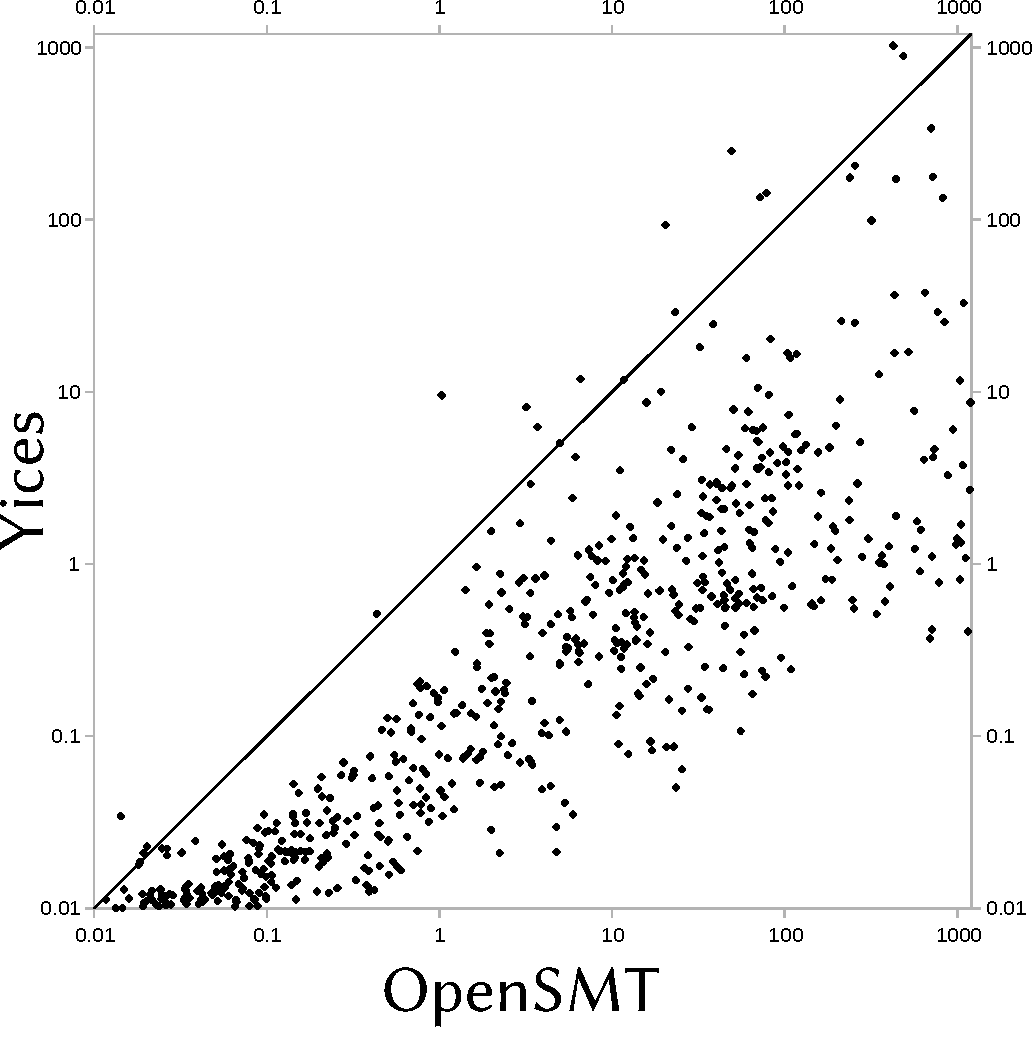
\includegraphics[width=0.49\linewidth]{comp_yices}
		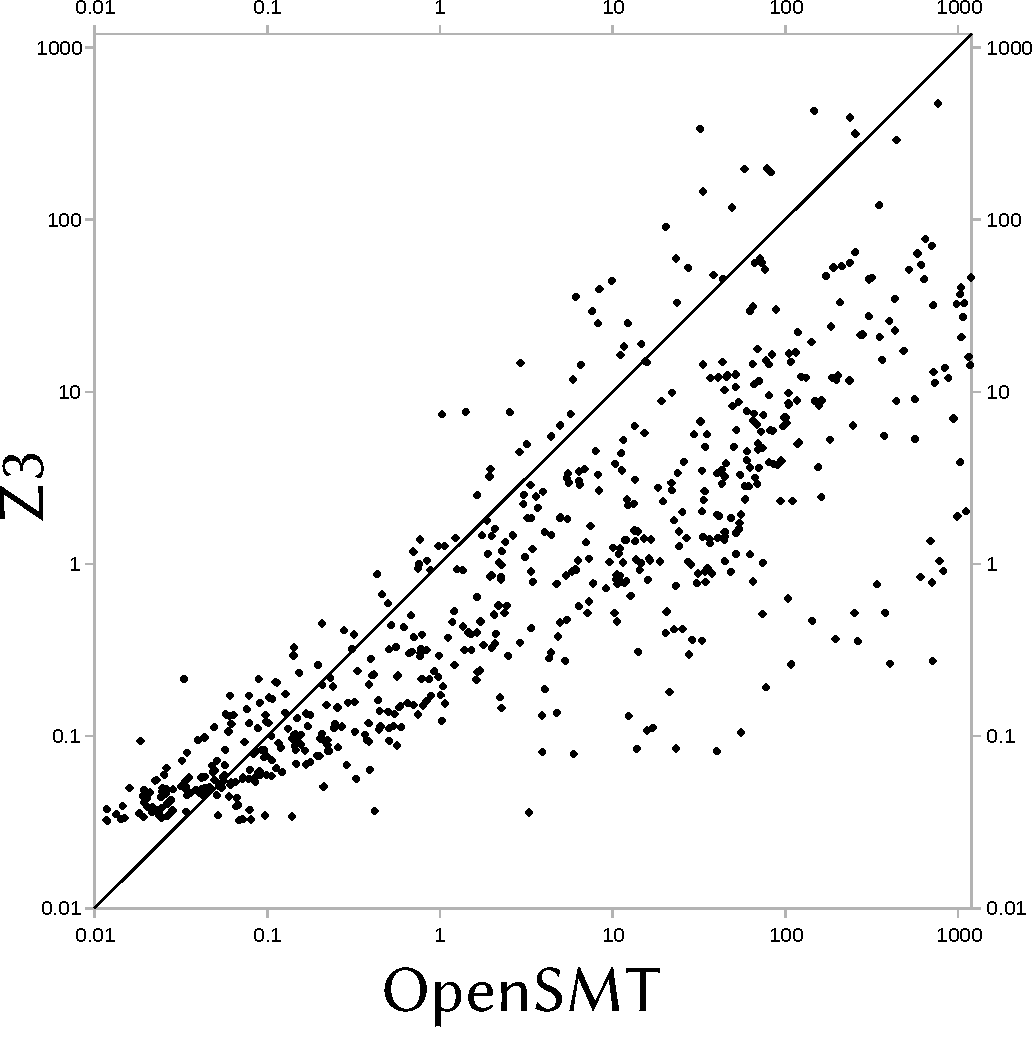
\includegraphics[width=0.49\linewidth]{comp_z3}\\
		\vspace{5px}
		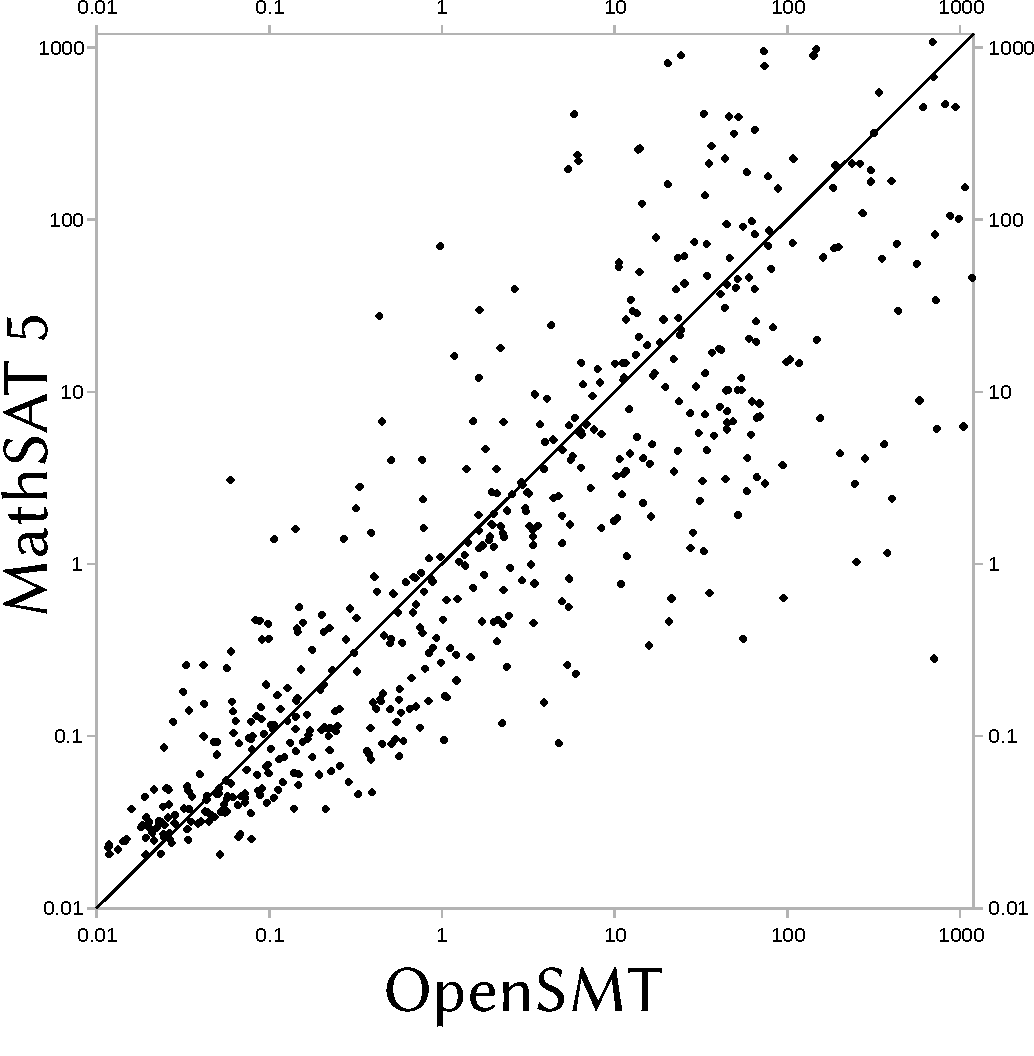
\includegraphics[width=0.49\linewidth]{comp_mathsat}
		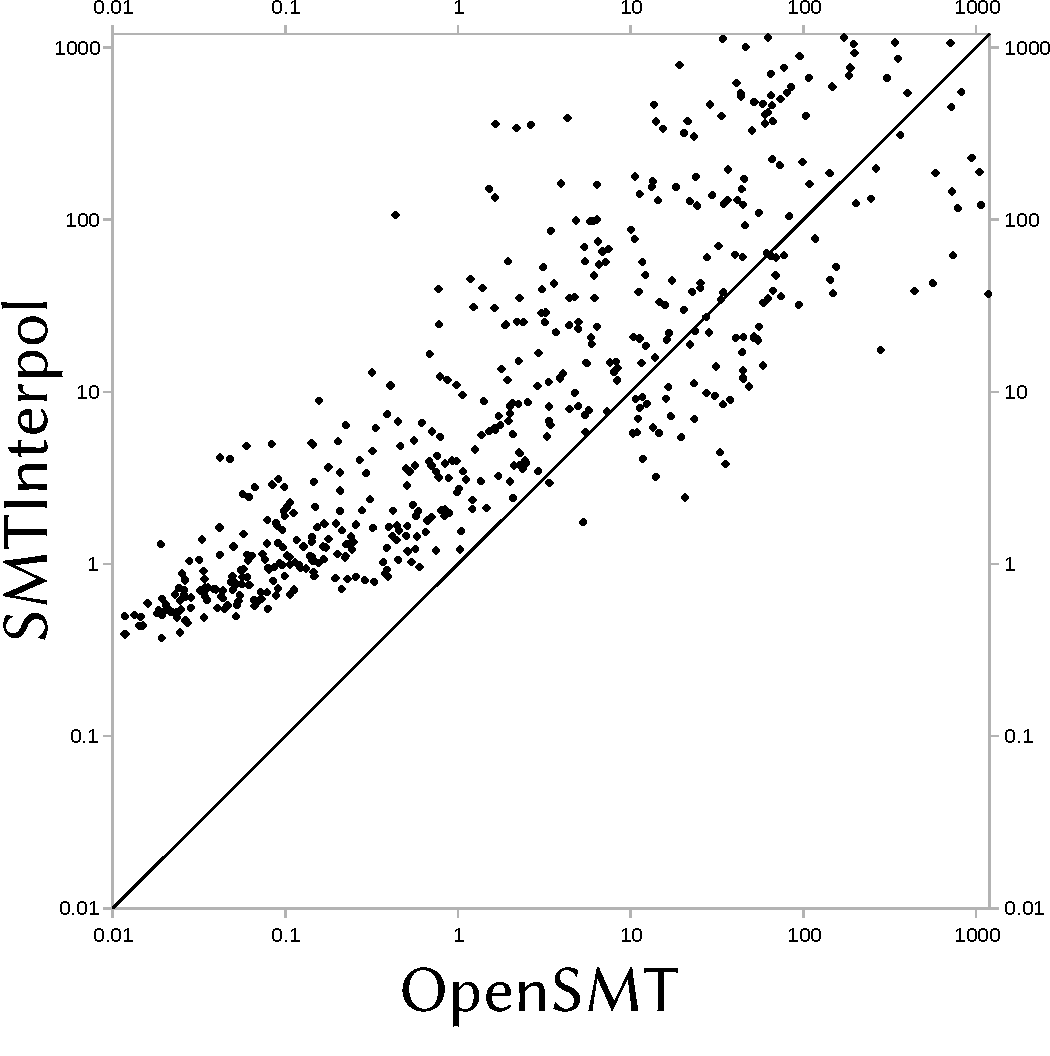
\includegraphics[width=0.49\linewidth]{comp_smti}\\
		\vspace{5px}
		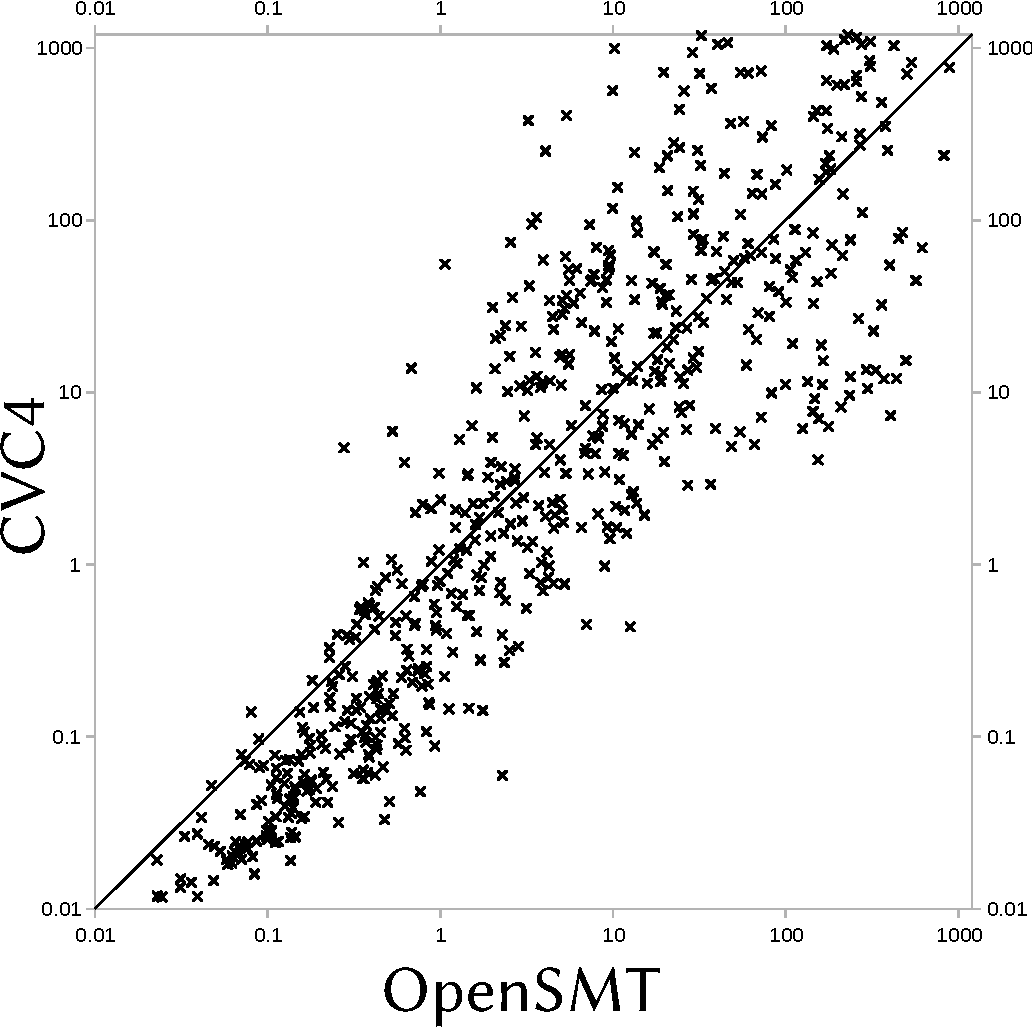
\includegraphics[width=0.49\linewidth]{comp_cvc}
		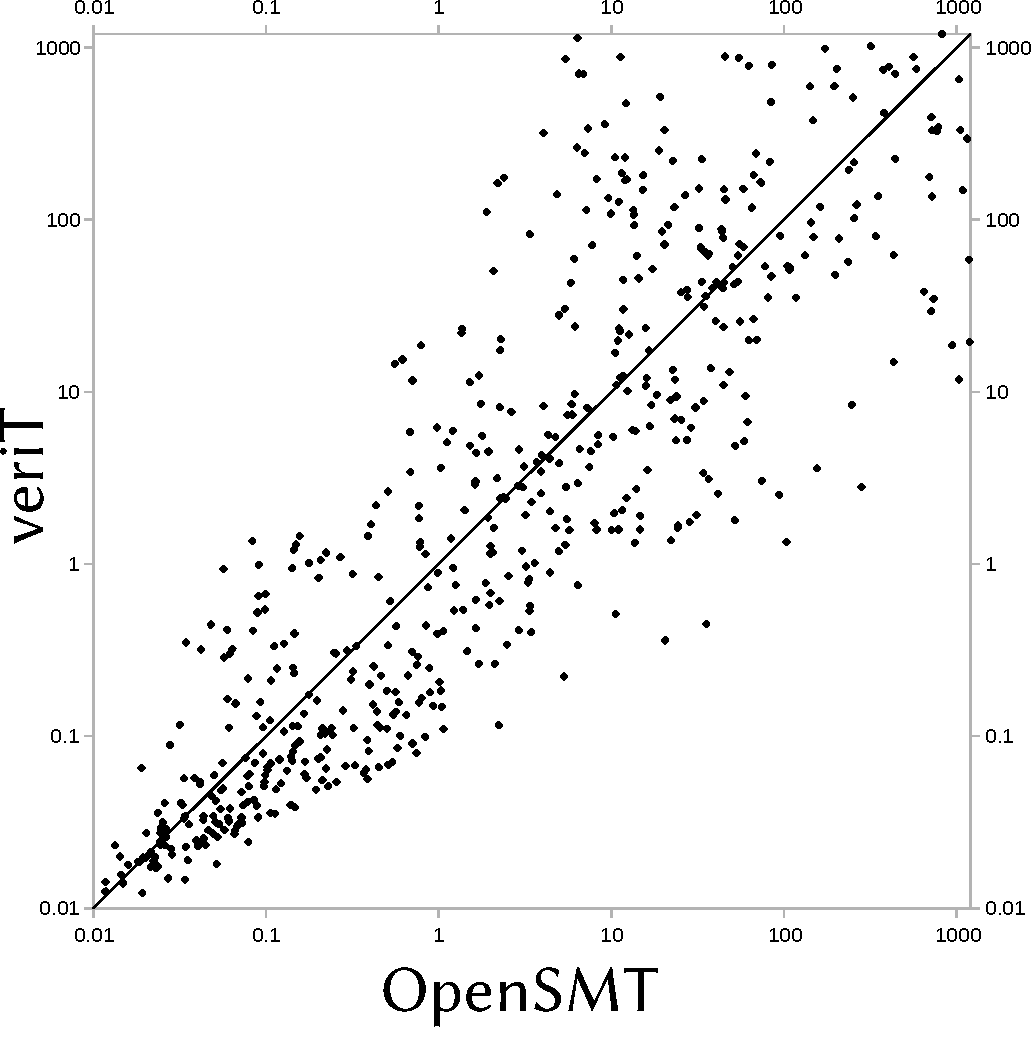
\includegraphics[width=0.49\linewidth]{comp_verit}
}
\section{Srovnání}
